% ============================================================
%  CHAPITRE 2 — Section : Analyse de sensibilité & coût total unifié (VoLL)
% ============================================================

\section{Analyse de sensibilité \& coût total unifié}
\label{sec:sensibilite}

L'ensemble des résultats présentés jusqu'ici découle d'une simulation déterministe unique, conduite avec des paramètres nominaux. La pertinence du classement des stratégies, et en particulier le statut de meilleure stratégie statique attribué à RB2, doit donc être confrontée à l'incertitude qui entache les principales hypothèses de modélisation. Cette section répond à cette exigence en plusieurs temps~: deux vérifications spécifiques (robustesse au bruit d'estimation du SoH, puis sensibilité à la résolution temporelle), une analyse de sensibilité de Monte-Carlo appliquée uniformément à l'ensemble des EMS, et enfin la réduction des deux objectifs à un \emph{coût total unifié} reposant sur une valeur de la charge non desservie, qui permet de classer les stratégies par un critère scalaire unique.

% ------------------------------------------------------------
\subsection{Robustesse de l'approche réactive au bruit d'estimation}
% ------------------------------------------------------------

Une première vérification concerne spécifiquement l'approche réactive au vieillissement, commune à toutes les EMS~: celle-ci agit sur le SoH \emph{estimé}, et non sur sa valeur réelle. Pour s'assurer que cette dépendance ne constitue pas une fragilité, un bruit d'estimation gaussien d'écart-type \SI{2}{\percent}, rafraîchi chaque semaine, est injecté sur l'estimation du SoH utilisée pour actualiser les plages de fonctionnement. Les performances restent alors très proches du cas à information exacte~: l'actualisation réactive des limites physiques se révèle essentiellement insensible à un bruit d'estimation réaliste, et le classement des stratégies n'en est pas affecté. Ce résultat conforte l'hypothèse, posée à la section~\ref{sec:soh}, selon laquelle les méthodes d'estimation existantes sont suffisamment précises pour les besoins du contrôle.

% ------------------------------------------------------------
\subsection{Sensibilité à la résolution temporelle}
% ------------------------------------------------------------

Une seconde vérification porte sur le pas d'échantillonnage. Toutes les simulations précédentes ont été conduites à pas horaire, qui néglige par construction les variations infra-horaires de la production PV et de la demande, et donc une partie des sollicitations rapides des composants. Pour éprouver ce choix, la stratégie de référence RB2 est resimulée sur l'horizon complet à un pas de \SI{10}{\minute}, en injectant sur les profils PV et de charge un bruit gaussien intra-horaire d'écart-type $\sigma \in \{0,5,10,15\}\,\%$ de la valeur horaire, la moyenne horaire étant préservée de sorte que le bilan énergétique et les décisions de l'EMS restent inchangés.

Sans bruit, la simulation à \SI{10}{\minute} reproduit fidèlement la simulation horaire (coût de dégradation $65{,}4 \rightarrow 65{,}9$~k€, LPSP $\approx \SI{2{,}45}{\percent}$). La restitution des variations intra-horaires accroît en revanche le coût de dégradation de façon monotone avec l'amplitude du bruit, jusqu'à environ $+\SI{15}{\percent}$ à $\sigma = \SI{15}{\percent}$ ($65{,}4 \rightarrow 75{,}2$~k€)~: la résolution horaire sous-estime donc légèrement la dégradation. La LPSP reste quant à elle quasiment inchangée ($\approx \SI{2{,}45}{\percent}$), et la hiérarchie des mécanismes de dégradation (en particulier la prééminence des cycles de démarrage-arrêt) est préservée à tous les pas et amplitudes. Le pas horaire constitue ainsi une estimation \emph{conservatrice} (borne inférieure) de la dégradation, sans remettre en cause les conclusions tirées du classement des stratégies.

% ------------------------------------------------------------
\subsection{Analyse de sensibilité de Monte-Carlo}
% ------------------------------------------------------------

Au-delà de cette vérification spécifique, les incertitudes de modélisation restantes affectent toutes les stratégies de la même manière~; elles sont donc évaluées par des analyses de sensibilité de Monte-Carlo appliquées uniformément à l'ensemble des EMS. Quatre familles d'incertitude sont considérées~:
\begin{itemize}
  \setlength\itemsep{2pt}
  \item les \textbf{critères de fin de vie} (EoL) des trois composants~: SoH de fin de vie de la batterie tiré dans $[0{,}60\,;\,0{,}80]$, et des composants hydrogène dans $[0{,}85\,;\,0{,}95]$~;
  \item les \textbf{seuils de la fonction de dégradation} des composants hydrogène, c'est-à-dire les seuils de régime du modèle de dégradation par morceaux, chacun échantillonné à $\pm\SI{20}{\percent}$ de sa valeur nominale~;
  \item les \textbf{poids de coût de remplacement} qui pondèrent la contribution de chaque composant à l'axe des coûts, chacun varié de $\pm\SI{30}{\percent}$ (la LPSP étant invariante à ces poids, cet échantillonnage se réduit à une dilatation analytique de l'axe des coûts)~;
  \item le \textbf{dimensionnement des composants}, les puissances/capacités de la batterie, de la pile à combustible et de l'électrolyseur étant chacune multipliées par un facteur indépendant tiré uniformément dans $[0{,}80\,;\,1{,}20]$, le champ PV étant laissé inchangé.
\end{itemize}
Chaque famille repose sur $N = 200$ tirages, les mêmes étant réutilisés pour toutes les stratégies afin que la comparaison ne soit pas polluée par le bruit d'échantillonnage. Chaque tirage est propagé à travers une simulation complète de vingt-cinq ans, fournissant pour chaque stratégie un résultat bidimensionnel (LPSP et coût de dégradation). Le Tableau~\ref{tab:sensitivity} en résume les plages et les conclusions, et la Figure~\ref{fig:sens_eol} en illustre un exemple (échantillonnage des critères de fin de vie) sous forme de nuage de points dans le plan de Pareto, assorti d'ellipses de dispersion.

\begin{table}[h!]
\centering
\caption{Analyses de sensibilité~: plages de perturbation et conclusions. Le classement des stratégies est préservé dans tous les cas.}
\label{tab:sensitivity}
\footnotesize
\renewcommand{\arraystretch}{1.25}
\begin{tabularx}{\textwidth}{p{3.3cm} X X}
\hline
\textbf{Analyse} & \textbf{Paramètre(s) et plage} & \textbf{Conclusion} \\ \hline
Erreur d'estimation du SoH & Bruit gaussien $\sigma = \SI{2}{\percent}$, rafraîchi chaque semaine & Performances quasi inchangées~; classement préservé. \\
Poids de coût & $\pm\SI{30}{\percent}$ sur les trois poids de remplacement & LPSP invariante~; coût linéaire en les poids~; classement inchangé (coût RB2 $65{,}6$~k€, IC~95\,\% $[51{,}3\,;\,80{,}0]$). \\
Critères de fin de vie & Batterie $[0{,}60\,;\,0{,}80]$, PAC/ELY $[0{,}85\,;\,0{,}95]$ & Effet marqué sur le coût absolu (durée de vie batterie $5{,}5 \rightarrow 2{,}5$~ans) mais classement inchangé (coût RB2 $62{,}6 \pm 9{,}5$~k€). \\
Seuils de dégradation PEM & Les quatre seuils de régime, chacun $\pm\SI{20}{\percent}$ & Classement inchangé~; coût RB2 $65{,}4 \rightarrow 66{,}9 \pm 9{,}7$~k€. \\
Dimensionnement & Calibres BAT/PAC/ELY $\times[0{,}80\,;\,1{,}20]$, PV fixe & Les deux axes se déplacent (batterie plus grande $\rightarrow$ LPSP plus faible, coût plus élevé) mais classement inchangé~; RB2 reste favorable (dég. $64{,}6 \pm 4{,}2$~k€, LPSP $3{,}06 \pm 0{,}79\,\%$). \\
Résolution temporelle & $T_s = \SI{10}{\minute}$ vs $\SI{1}{\hour}$~; bruit gaussien intra-horaire sur PV \& charge, $\sigma \in \{0,5,10,15\}\,\%$ (moyenne horaire préservée) & Seul le coût de dégradation croît avec le bruit (RB2 $65{,}4 \rightarrow 75{,}2$~k€)~; LPSP $\approx \SI{2{,}45}{\percent}$ et hiérarchie des mécanismes inchangées. \\ \hline
\end{tabularx}
\end{table}
\FloatBarrier

\begin{figure}[h!]
    \centering
    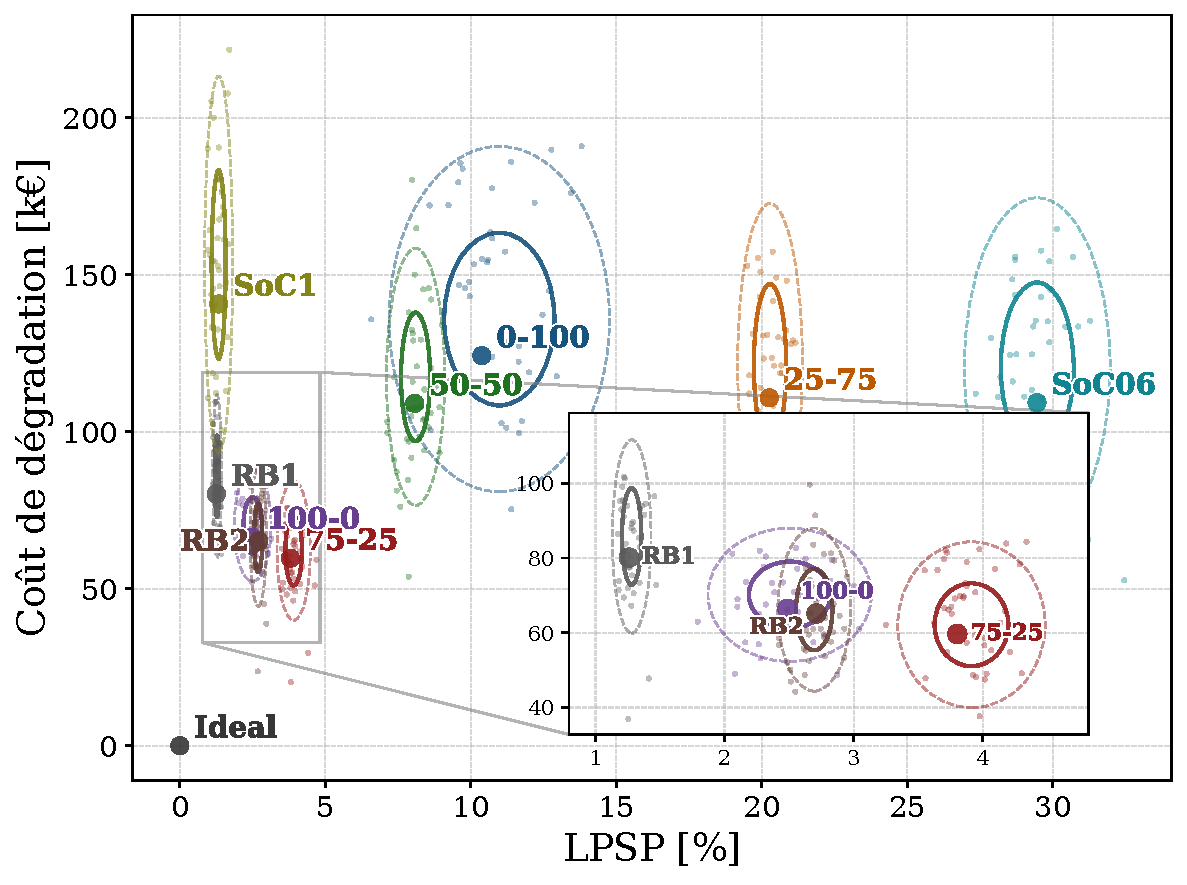
\includegraphics[width=0.8\linewidth]{Chapitre 2/Sensibilite/Figures/sens_eol_pareto.pdf}
    \caption{Plan de Pareto sous échantillonnage de Monte-Carlo des critères de fin de vie (ellipses de dispersion à $1\sigma$ en trait plein et $2\sigma$ en pointillés).}
    \label{fig:sens_eol}
\end{figure}
\FloatBarrier

Deux conclusions robustes se dégagent. Premièrement, chaque perturbation se contente, pour l'essentiel, de \emph{redimensionner} les indicateurs absolus sans rebattre l'ordre des stratégies~: les perturbations de poids et de seuils dilatent principalement l'axe des coûts, les critères de fin de vie en déplacent en outre le niveau absolu (la durée de vie de la batterie variant de $5{,}5$ à $2{,}5$~ans), et la perturbation de dimensionnement déplace les deux axes (une batterie plus grande abaissant la LPSP au prix d'un coût de dégradation supérieur). Dans tous les cas, RB2 conserve sa position favorable et non dominée. Le cas du dimensionnement mérite un commentaire spécifique~: la configuration nominale (un champ PV surdimensionné par rapport à la charge, d'où un électrolyseur surdimensionné et une pile à combustible sous-dimensionnée) découle directement des profils de terrain du cas d'étude~; la perturbation de $\pm\SI{20}{\percent}$ confirme que le classement reflète la logique de contrôle et non ce point de dimensionnement particulier.

% ------------------------------------------------------------
\subsection{Critère de coût total unifié (VoLL)}
% ------------------------------------------------------------

Comparer les stratégies sur chaque plan de Pareto bidimensionnel est instructif mais fastidieux, d'autant que les deux objectifs sont exprimés dans des unités différentes (un pourcentage et un coût). Un critère plus concis et plus directement objectivable consiste à réduire le résultat à un scalaire unique, en attribuant une valeur monétaire à la charge non desservie au moyen d'une \emph{valeur de la charge perdue} (VoLL, \textit{Value of Lost Load}), ajoutée au coût de dégradation~\cite{keskinis_techno-economic_2025}~:
\begin{equation}
    C_{\text{tot}} = C_{\text{deg}} + \mathrm{VoLL} \times E_{\text{non servie}}
    \label{eq:total_cost}
\end{equation}
où $E_{\text{non servie}} = \mathrm{LPSP} \times E_{\text{planifiée}}$ est l'énergie que les usagers prévoyaient de consommer mais que le système n'a pu fournir sur l'ensemble de l'horizon, $E_{\text{planifiée}}$ étant l'énergie de charge nette planifiée et LPSP la probabilité de perte d'alimentation. Conformément à la pratique courante en évaluation de fiabilité des micro-réseaux, la VoLL est maintenue constante et fixée à $\mathrm{VoLL} = 3~\text{€/kWh}$, valeur médiane représentative d'une charge résidentielle mixte~\cite{CEPA2018VoLL}\cite{jin_evaluating_2025}. Ce choix conditionne l'arbitrage entre les deux objectifs~: une VoLL faible privilégie les stratégies sobres en dégradation, tandis qu'une VoLL élevée favoriserait celles qui minimisent la LPSP (RB1, SoC1). Pour la valeur retenue, intermédiaire, le classement reste stable et RB2 conserve sa position de tête (Fig. \ref{fig:ranking}). Le scalaire unique $C_{\text{tot}}$ rend les stratégies directement comparables, aussi bien à l'intérieur de chaque cas de sensibilité qu'entre les différents cas.

La réduction de chaque résultat au scalaire $C_{\text{tot}}$ produit le classement unifié de la Figure~\ref{fig:ranking}. RB2 obtient le \textbf{meilleur rang moyen} ($1{,}2$ sur l'ensemble des cas) et se classe première dans quatre des cinq cas de sensibilité (nominal, critères de fin de vie, poids de coût et dimensionnement). Elle n'est devancée que sur le seul cas des seuils de dégradation des composants hydrogène, où la stratégie « tout-batterie » 100-0 réalise le coût total le plus faible. Ces deux stratégies sont d'ailleurs très rapprochées (rang moyen $1{,}2$ pour RB2 contre $1{,}8$ pour 100-0) et devancent nettement les suivantes (RB1 puis 75-25), tandis que les stratégies très coûteuses en dégradation (SoC1) ou à forte LPSP (50-50, 0-100, 25-75 et surtout SoC06) ferment la marche dès lors que la charge non desservie est valorisée. RB2 demeure ainsi la stratégie la plus régulièrement performante, sans être strictement dominante~: ce point de vue scalaire confirme et nuance à la fois le verdict du plan de Pareto nominal. Il est à noter que ce constat est lui même dépendant de la valeur de VoLL fixée, et dans ce cas RB2 reste la stratégie la plus performante jusqu'à une valeur de 5,2€/kWh, au-delà de laquelle RB1 devient la stratégie la plus intéressante.

\begin{figure}[h!]
    \centering
    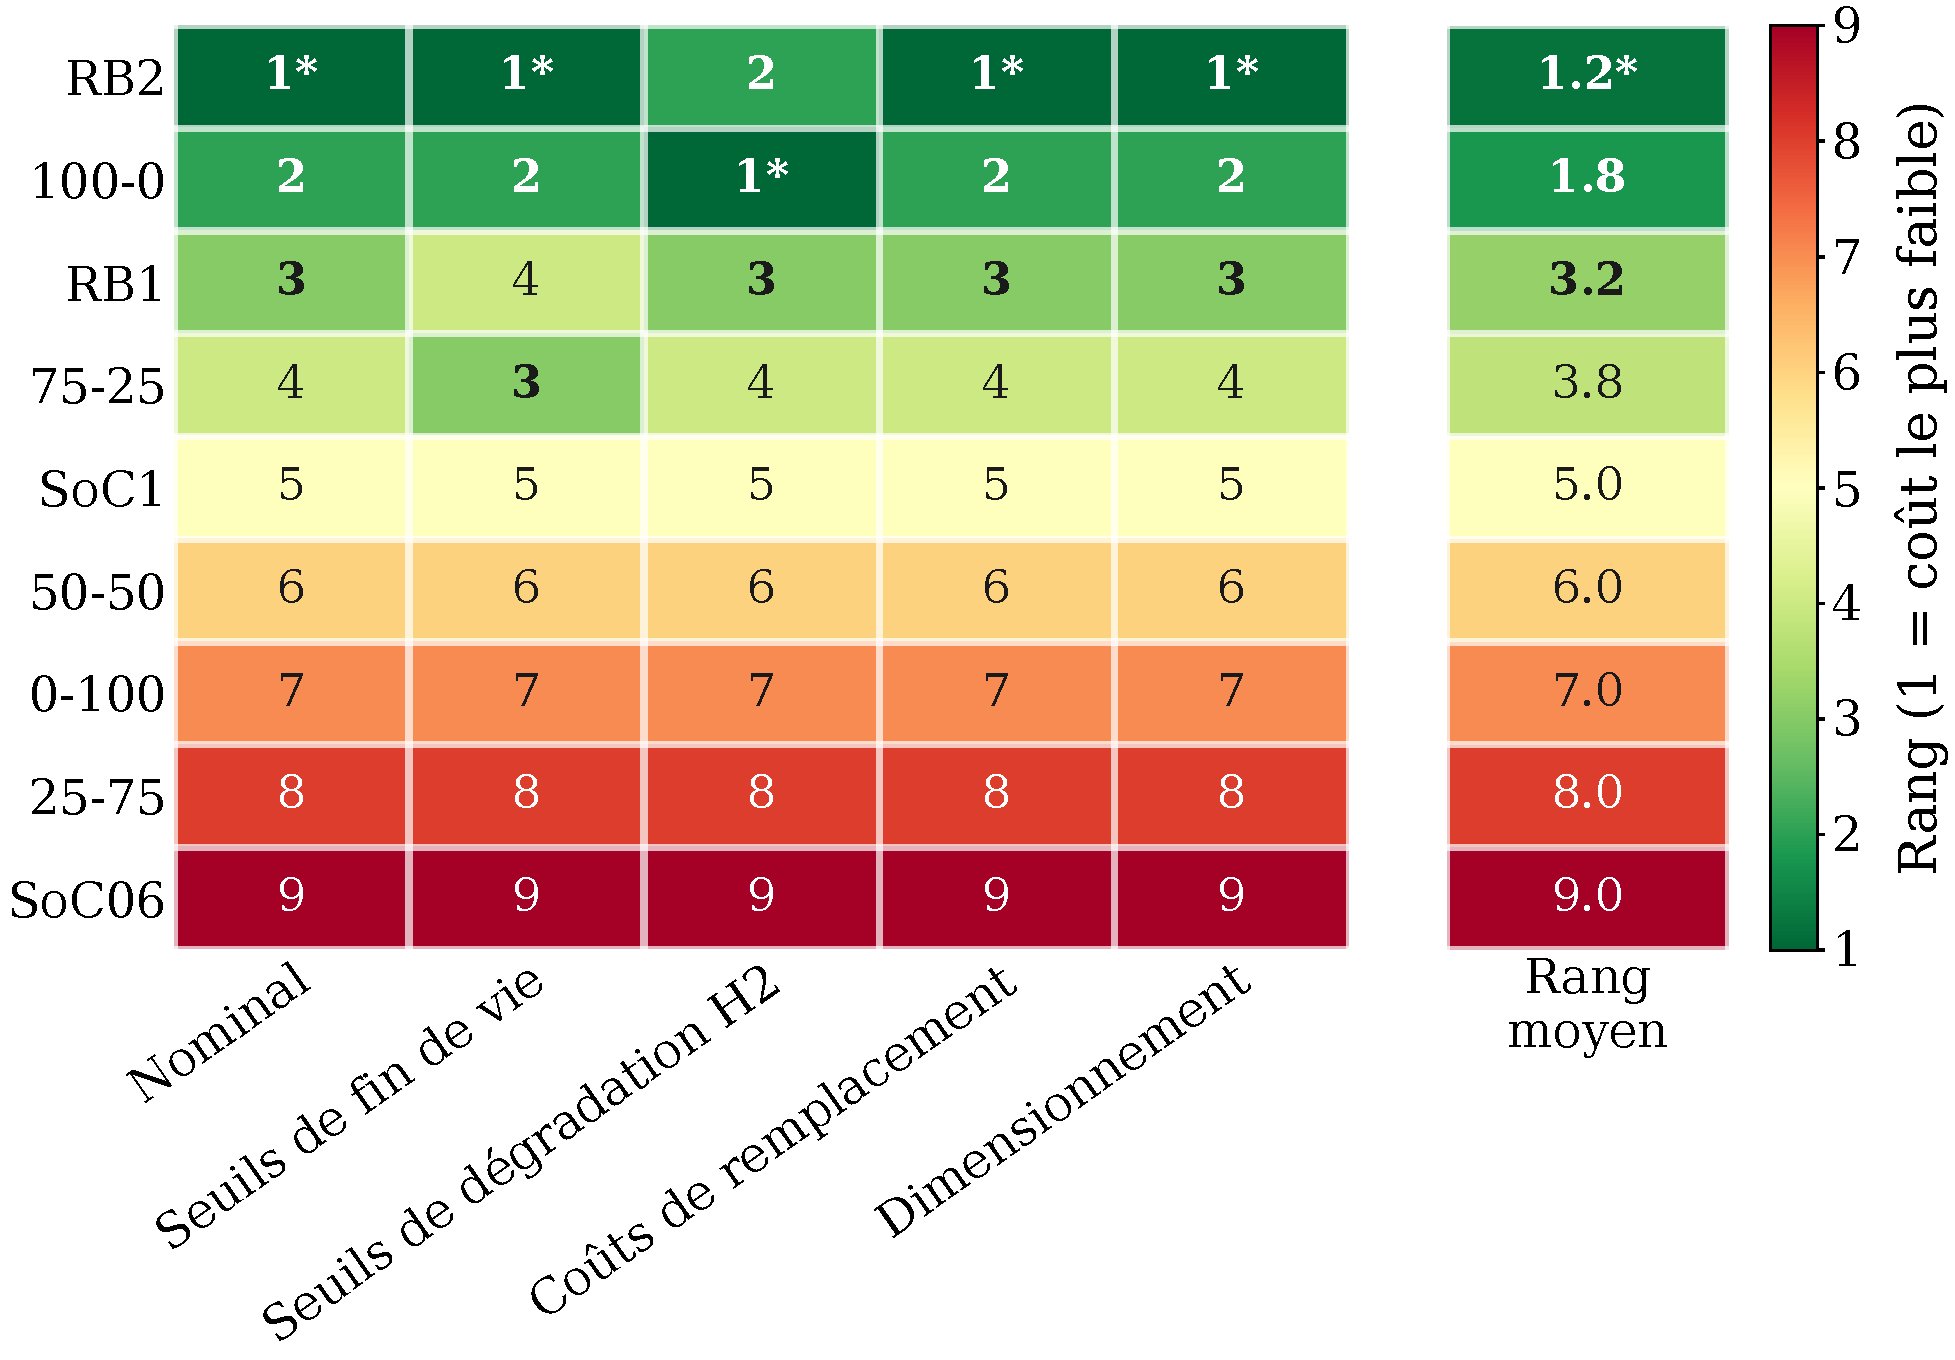
\includegraphics[width=\linewidth]{Chapitre 2/Sensibilite/Figures/voll_ranking_fr.pdf}
    \caption{Classement unifié par le coût total $C_{\text{tot}}$ à travers les cas de sensibilité.}
    \label{fig:ranking}
\end{figure}
\FloatBarrier

Au sens du coût total unifié, RB2 apparaît donc comme la stratégie statique la plus régulièrement performante, et ce de manière cohérente sur toute la gamme des hypothèses de modélisation et de dimensionnement testées. Ce constat consolide le choix de RB2 comme stratégie de référence et ouvre la voie à son amélioration au chapitre suivant.